\chapter{Chapter \ref{ChapterConversations} Voice Guidance and Conversations}
\label{AppendixB}

These are the voice guidance and conversations played to the participants when evaluating the voice-based technique described in Chapter \ref{ChapterConversations}. 

\begin{table}[h]
\centering
\caption{Voice guidance for the Familiarity route in Japanese and Filipino languages.}~\label{tab:b-fami}
\begin{tabular}{ll}
\hline
\multicolumn{2}{l}{English}                            \\ \hline
1. & Let's get started!                                \\
2. & In 500 meters, turn left.                         \\
3. & Go straight.                                      \\
4. & In 500 meters, turn left and then turn right.     \\
5. & You've arrived at your destination.               \\ \hline
   &                                                   \\ \hline
\multicolumn{2}{l}{Japanese}                           \\ \hline
1. & 案内を開始します                                          \\
2. & 500メートル先で左折です。                                    \\
3. & 直進です。                                             \\
4. & 500メートル先で左折、その後右折です。                              \\
5. & 目的地に到着しました。                                       \\ \hline
   &                                                   \\ \hline
\multicolumn{2}{l}{Filipino}                           \\ \hline
1. & Magsimula na tayo                                 \\
2. & Kumaliwa pagkatapos ng 500 metro.                 \\
3. & Deretso lang.                                     \\
4. & Pagkalagpas ng 500 metro, kumaliwa tapos kumanan. \\
5. & Nakarating na tayo sa destinasyon.                \\ \hline
\end{tabular}
\end{table}

\begin{figure}[h]
  \centering
  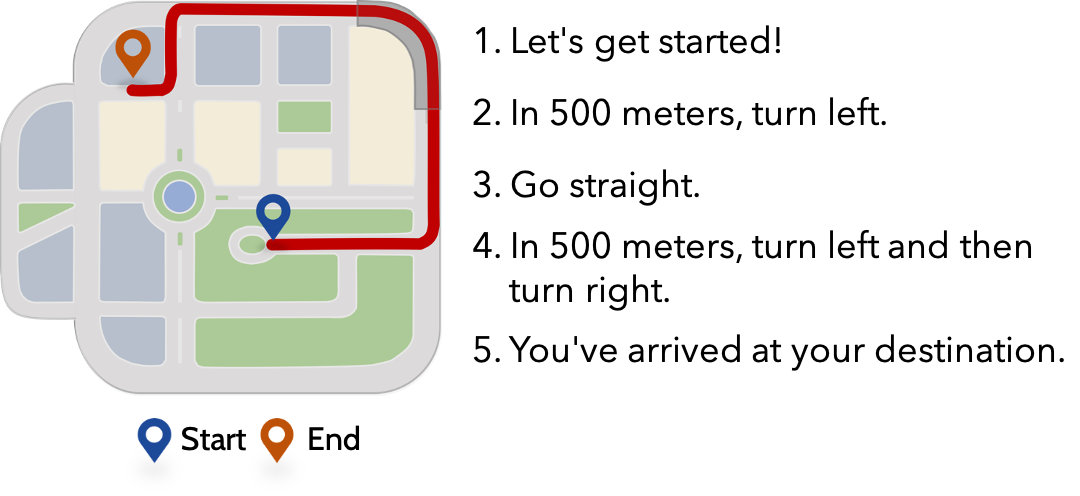
\includegraphics[scale=0.7]{figures/b-familiarity-en.png}
  \caption{The Familiarity route and the voice guidance in English.}
  \label{fig:b-fami}
\end{figure}

\begin{table}[h]
\centering
\caption{Voice guidance for the Familiar route (Route F in Figure \ref{fig:b-all-routes}) in three languages.}~\label{tab:b-familiar-pure}
\begin{tabular}{ll}
\hline
\multicolumn{2}{l}{English}                                                                                            \\ \hline
1. & Let's get started!                                                                                                \\
2. & Let's turn left after 500 meters. \\ 
   & We take that direction on most days. \\
3. & Let's continue straight. \\ 
   & We always go through the tunnel.              \\
4. & Let's turn left after 500 meters and then turn right. \\ 
   & We usually take that turn near our destination. \\
5. & We've arrived at our destination.                                                                                 \\ \hline
   &                                                                                                                   \\ \hline
\multicolumn{2}{l}{Japanese}                                                                                           \\ \hline
1. & 案内を開始します                                                                                                          \\
2. & 500メートル進んだ先を左折です。\\ 
   & いつもこの道を通りますよね。                                      \\
3. & 直進を続けてください。\\ 
   & そのトンネルをよく通っていますよね。                                          \\
4. & 500メートル先を左折、その後右折です。\\ 
   & いつもどおりの行き方で目的地に行きましょう。                           \\
5. & 目的地に到着しました。                                                                                                      \\ \hline
   &                                                                                                                   \\ \hline
\multicolumn{2}{l}{Filipino}                                                                                           \\ \hline
1. & Magsimula na tayo                                                                                                 \\
2. & Kumaliwa tayo pagkatapos ng 500 metro. \\ 
   & Madalas nating dinadaanan yan.  \\
3. & Dumeretso tayo. Lagi tayong dumadaan sa ilalim ng tunnel.                                                         \\
4. & Kumaliwa tayo pagkatapos ng 500 metro tapos kanan. \\ 
   & Ganyan ang daan natin pag malapit na tayo.         \\
5. & Nakarating na tayo sa ating destinasyon.                                                                          \\ \hline
\end{tabular}
\end{table}

\begin{figure}[h]
  \centering
  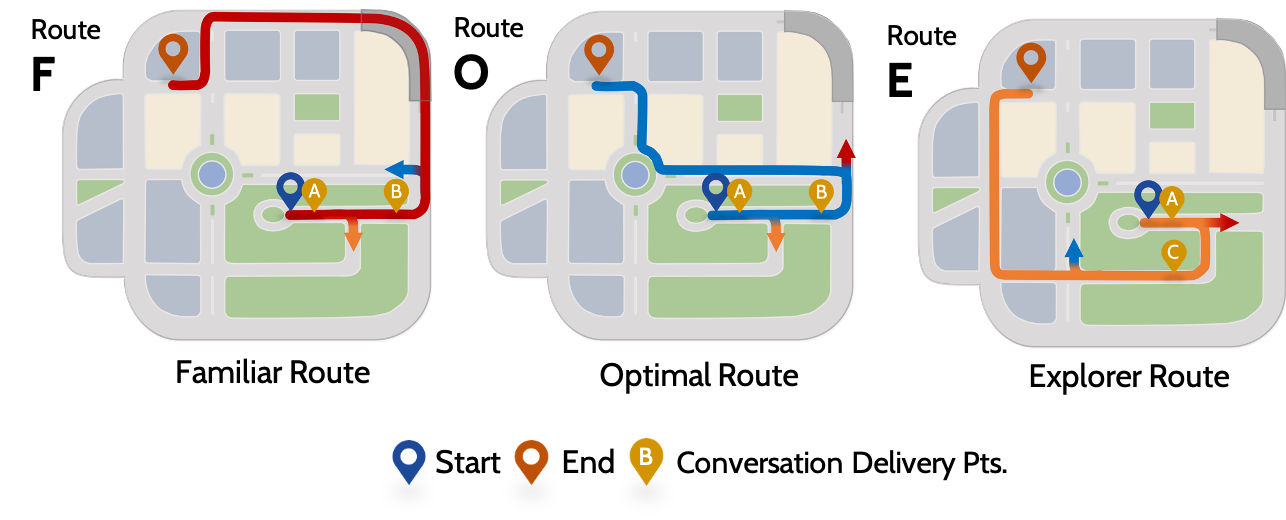
\includegraphics[scale=0.6]{figures/s2-all-routes.png}
  \caption{The different routes used for the voice-based technique described in Chapter \ref{ChapterConversations}.}
  \label{fig:b-all-routes}
\end{figure}

\begin{table}[h]
\centering
\caption{Voice guidance for the Optimal route (Route O in Figure \ref{fig:b-all-routes}) in three languages.}~\label{tab:b-optimal-pure}
\begin{tabular}{ll}
\hline
\multicolumn{2}{l}{English}                                        \\ \hline
1. & Let's get started!                                            \\
2. & Let's turn left after 500 meters.                             \\
3. & We can turn left again in 300 meters. It will take us faster. \\
4. & Let's go straight to the roundabout and take the first exit.  \\
   & There are less traffic signals to wait for.                   \\
5. & Let's turn left after 500 meters.                             \\
6. & We've arrived at our destination.                             \\ \hline
   &                                                               \\ \hline
\multicolumn{2}{l}{Japanese}                                       \\ \hline
1. & 案内を開始します                                                      \\
2. & 500メートル先で左折です。                                                \\
3. & 再び、左折してください。こちらだと早く着くでしょう。                                    \\
4. & 直進しラウンドアバウトの最初の出口を出ましょう。                                      \\
   & こちらだと信号待ちが少ないです。                                              \\
5. & 500メートル先左折です。                                                 \\
6. & 目的地に到着しました。                                                   \\ \hline
   &                                                               \\ \hline
\multicolumn{2}{l}{Filipino}                                       \\ \hline
1. & Magsimula na tayo                                             \\
2. & Kumaliwa tayo pagkatapos ng 500 metro.                        \\
3. & Kumaliwa tayo ulit bago mag-tunnel. Mas mabilis doon.         \\
4. & Dumeretso tayo sa rotonda at lumabas sa unang exit.           \\
   & Mas kaunti hihintayin nating stop light.                      \\
5. & Kumaliwa tayo pagkatapos ng 500 metro.                        \\
6. & Nakarating na tayo sa ating destinasyon.                      \\ \hline
\end{tabular}
\end{table}

\begin{table}[h]
\centering
\caption{Voice guidance for the Explorer route (Route E in Figure \ref{fig:b-all-routes}) in three languages.}~\label{tab:b-explorer-pure}
\begin{tabular}{ll}
\hline
\multicolumn{2}{l}{English}                                                  \\ \hline
1. & Let's get started!                                                      \\
2. & Let's turn right. I think we haven't gone in this direction before.     \\
3. & Let's turn right in 500 meters. We should see a new part of town there. \\
4. & Let's turn right after 500 meters to our destination.                   \\
5. & We've arrived at our destination.                                       \\ \hline
   &                                                                         \\ \hline
\multicolumn{2}{l}{Japanese}                                                 \\ \hline
1. & 案内を開始します                                                                \\
2. & 右折しましょう。この方向には行ったことがないと思います。                                            \\
3. & 500メートル先を右折です。                                                          \\
   & 私たちは町の新しい所を見るのも良いでしょう。                                                  \\
4. & 500メートル先、右折です。                                                          \\
5. & 目的地に到着しました。                                                             \\ \hline
   &                                                                         \\ \hline
\multicolumn{2}{l}{Filipino}                                                 \\ \hline
1. & Magsimula na tayo                                                       \\
2. & Kumanan tayo. Hindi pa yata tayo nakakadaan dito dati.                  \\
3. & Kumanan tayo pagkatapos ng 500 metro.                                   \\
   & Puwede natin makita yung kabilang banda ng barangay dun.                \\
4. & Kumanan tayo pagkatapos ng 500 metro papunta sa ating destinasyon.      \\
5. & Nakarating na tayo sa ating destinasyon.                                \\ \hline
\end{tabular}
\end{table}

\begin{table}[h]
\centering
\caption{Voice guidance when the Familiar + Optimal conversation is played.}~\label{tab:b-FO}
\begin{tabular}{ll}
\hline
\multicolumn{2}{l}{English}                                                                      \\ \hline
1.                      & Let's get started!                                                     \\
2.                      & Let's turn left after 500 meters. We take that direction on most days. \\ \hline
\multicolumn{1}{|l}{3.} & \multicolumn{1}{l|}{F: Let's continue straight.}                       \\
\multicolumn{1}{|l}{4.} & \multicolumn{1}{l|}{O: We can also turn left before the tunnel.}                    \\
\multicolumn{1}{|l}{5.} & \multicolumn{1}{l|}{F: But we always go through the tunnel.}                        \\
\multicolumn{1}{|l}{6.} & \multicolumn{1}{l|}{O: Yes, but turning left will take us faster.}                  \\ \hline
\multicolumn{2}{l}{\textit{continue voice guidance based on what was chosen...}}                              \\
                        &                                                                        \\ \hline
\multicolumn{2}{l}{Japanese}                                                                     \\ \hline
1.                      & 案内を開始します                                                               \\
2.                      & 500メートル先を左折です。いつもその道を通りますよね。                                           \\ \hline
\multicolumn{1}{|l}{3.} & \multicolumn{1}{l|}{F: そのまま直進してください。}                                  \\
\multicolumn{1}{|l}{4.} & \multicolumn{1}{l|}{O:トンネルの前で左折することもできます。}                             \\
\multicolumn{1}{|l}{5.} & \multicolumn{1}{l|}{F: でもいつもよくトンネルを通っていますよね。}                          \\
\multicolumn{1}{|l}{6.} & \multicolumn{1}{l|}{O: はい、でも左折すると早くなります。}                              \\ \hline
\multicolumn{2}{l}{continue voice guidance based on what was chosen...}                          \\
                        &                                                                        \\ \hline
\multicolumn{2}{l}{Filipino}                                                                     \\ \hline
1.                      & Magsimula na tayo                                                      \\
2.                      & Kumaliwa tayo pagkatapos ng 500 metro. Madalas nating dinadaanan yan.  \\ \hline
\multicolumn{1}{|l}{3.} & \multicolumn{1}{l|}{F: Dumeretso tayo.}                                \\
\multicolumn{1}{|l}{4.} & \multicolumn{1}{l|}{O: Alam mo, puwede rin tayo kumaliwa bago mag-tunnel.}          \\
\multicolumn{1}{|l}{5.} & \multicolumn{1}{l|}{F: Oo, pero hindi ba lagi tayong dumadaan sa ilalim ng tunnel.} \\
\multicolumn{1}{|l}{6.} & \multicolumn{1}{l|}{O: Tama ka, pero mas mabilis pag kumaliwa tayo.}                \\ \hline
\multicolumn{2}{l}{continue voice guidance based on what was chosen...}                          \\ \hline
\end{tabular}
\end{table}

\begin{table}[h]
\centering
\caption{Voice guidance when the Familiar + Explorer conversation is played.}~\label{tab:b-FE}
\begin{tabular}{ll}
\hline
\multicolumn{2}{l}{English}                                                                           \\ \hline
1.                      & Let's get started!                                                          \\ \hline
\multicolumn{1}{|l}{2.} & \multicolumn{1}{l|}{F: Let's go straight and then turn left.}               \\
\multicolumn{1}{|l}{3.} & \multicolumn{1}{l|}{E: How about turning right before that?}                \\
\multicolumn{1}{|l}{4.} & \multicolumn{1}{l|}{F: That's possible. But we take a left on most days.}   \\
\multicolumn{1}{|l}{5.} & \multicolumn{1}{l|}{E: That's true. But we haven't gone in this direction before.} \\ \hline
\multicolumn{2}{l}{\textit{continue voice guidance based on what was chosen...}}                      \\
                        &                                                                             \\ \hline
\multicolumn{2}{l}{Japanese}                                                                          \\ \hline
1.                      & 案内を開始します                                                                    \\ \hline
\multicolumn{1}{|l}{2.} & \multicolumn{1}{l|}{F: 直進してください、その後左折です。}                                   \\
\multicolumn{1}{|l}{3.} & \multicolumn{1}{l|}{E: 右折するのはどうですか?}                                        \\
\multicolumn{1}{|l}{4.} & \multicolumn{1}{l|}{F: それもいいんですけど、いつも左折しますよね。}                              \\
\multicolumn{1}{|l}{5.} & \multicolumn{1}{l|}{E: そうですね。しかし、この方向には行ったことがありません。}                        \\ \hline
\multicolumn{2}{l}{continue voice guidance based on what was chosen...}                               \\
                        &                                                                             \\ \hline
\multicolumn{2}{l}{Filipino}                                                                          \\ \hline
1.                      & Magsimula na tayo                                                           \\ \hline
\multicolumn{1}{|l}{2.} & \multicolumn{1}{l|}{F: Deretso lang tayo tapos kaliwa.}                     \\
\multicolumn{1}{|l}{3.} & \multicolumn{1}{l|}{E: Eh kung kumanan tayo bago yan?}                      \\
\multicolumn{1}{|l}{4.} & \multicolumn{1}{l|}{F: Puwede naman. Pero madalas doon pa tayo kumakaliwa.} \\
\multicolumn{1}{|l}{5.} & \multicolumn{1}{l|}{E: Totoo yan. Pero hindi pa tayo nakakadaan dito dati.} \\ \hline
\multicolumn{2}{l}{continue voice guidance based on what was chosen...}                               \\ \hline
\end{tabular}
\end{table}

\begin{table}[h]
\centering
\caption{Voice guidance when the Optimal + Familiar conversation is played.}~\label{tab:b-OF}
\begin{tabular}{ll}
\hline
\multicolumn{2}{l}{English}                                                            \\ \hline
1.                      & Let's get started!                                           \\
2.                      & Let's turn left after 500 meters.                            \\ \hline
\multicolumn{1}{|l}{3.} & \multicolumn{1}{l|}{O: Let's turn left again in 300 meters.} \\
\multicolumn{1}{|l}{4.} & \multicolumn{1}{l|}{F: How about we continue straight?}      \\
\multicolumn{1}{|l}{5.} & \multicolumn{1}{l|}{O: Turning left will take us there faster.}                       \\
\multicolumn{1}{|l}{6.} & \multicolumn{1}{l|}{F: Right. But don't we always go through the tunnel?}             \\ \hline
\multicolumn{2}{l}{\textit{continue voice guidance based on what was chosen...}}       \\
                        &                                                              \\ \hline
\multicolumn{2}{l}{Japanese}                                                           \\ \hline
1.                      & 案内を開始します                                                     \\
2.                      & 500メートル先左折です。                                                \\ \hline
\multicolumn{1}{|l}{3.} & \multicolumn{1}{l|}{O: 300メールでもう一度左折です。}                     \\
\multicolumn{1}{|l}{4.} & \multicolumn{1}{l|}{F: 直進はどうですか?}                            \\
\multicolumn{1}{|l}{5.} & \multicolumn{1}{l|}{O: 左折すると目的地に早く着きます。}                     \\
\multicolumn{1}{|l}{6.} & \multicolumn{1}{l|}{F: いいですね。でもいつもトンネルを通って行ってませんか?}          \\ \hline
\multicolumn{2}{l}{continue voice guidance based on what was chosen...}                \\
                        &                                                              \\ \hline
\multicolumn{2}{l}{Filipino}                                                           \\ \hline
1.                      & Magsimula na tayo                                            \\
2.                      & Kumaliwa tayo pagkatapos ng 500 metro.                       \\ \hline
\multicolumn{1}{|l}{3.} & \multicolumn{1}{l|}{O: Kumaliwa tayo ulit bago mag-tunnel.}  \\
\multicolumn{1}{|l}{4.} & \multicolumn{1}{l|}{F: Eh kung dumeretso kaya tayo?}         \\
\multicolumn{1}{|l}{5.} & \multicolumn{1}{l|}{O: Mas mabilis kung kakaliwa agad tayo.} \\
\multicolumn{1}{|l}{6.} & \multicolumn{1}{l|}{F: Tama. Pero hindi ba lagi tayong dumadaan sa ilalim ng tunnel?} \\ \hline
\multicolumn{2}{l}{continue voice guidance based on what was chosen...}                \\ \hline
\end{tabular}
\end{table}

\begin{table}[h]
\centering
\caption{Voice guidance when the Optimal + Explorer conversation is played.}~\label{tab:b-OE}
\begin{tabular}{ll}
\hline
\multicolumn{2}{l}{English}                                                             \\ \hline
1.                      & Let's get started!                                            \\ \hline
\multicolumn{1}{|l}{2.} & \multicolumn{1}{l|}{O: Let's go straight and then turn left.} \\
\multicolumn{1}{|l}{3.} & \multicolumn{1}{l|}{E: How about turning right before that?}  \\
\multicolumn{1}{|l}{4.} & \multicolumn{1}{l|}{O: I don't know about that. Going straight then left is a closer route.} \\
\multicolumn{1}{|l}{5.} & \multicolumn{1}{l|}{E: That's true. But we haven't gone in this direction before.}           \\ \hline
\multicolumn{2}{l}{\textit{continue voice guidance based on what was chosen...}}        \\
                        &                                                               \\ \hline
\multicolumn{2}{l}{Japanese}                                                            \\ \hline
1.                      & 案内を開始します                                                      \\ \hline
\multicolumn{1}{|l}{2.} & \multicolumn{1}{l|}{O: 直進して、それから左折です。}                        \\
\multicolumn{1}{|l}{3.} & \multicolumn{1}{l|}{E: 手前を右折したらどうですか。}                        \\
\multicolumn{1}{|l}{4.} & \multicolumn{1}{l|}{O: それは知りません。直進した後、左折すると近いです。}             \\
\multicolumn{1}{|l}{5.} & \multicolumn{1}{l|}{F: そうですね。しかし、この方向には行ったことがありません。}          \\ \hline
\multicolumn{2}{l}{continue voice guidance based on what was chosen...}                 \\
                        &                                                               \\ \hline
\multicolumn{2}{l}{Filipino}                                                            \\ \hline
1.                      & Magsimula na tayo                                             \\ \hline
\multicolumn{1}{|l}{2.} & \multicolumn{1}{l|}{O: Deretso tayo tapos kaliwa.}            \\
\multicolumn{1}{|l}{3.} & \multicolumn{1}{l|}{E: Kung kumanan kaya tayo bago yan?}      \\
\multicolumn{1}{|l}{4.} & \multicolumn{1}{l|}{O: Hindi ko alam. Mas malapit pag dumiretso tayo tapos kaliwa.}          \\
\multicolumn{1}{|l}{5.} & \multicolumn{1}{l|}{E: Tama. Pero hindi pa tayo nakakadaan dito dati.}                       \\ \hline
\multicolumn{2}{l}{continue voice guidance based on what was chosen...}                 \\ \hline
\end{tabular}
\end{table}

\begin{table}[h]
\centering
\caption{Voice guidance when the Explorer + Familiar conversation is played.}~\label{tab:b-EF}
\begin{tabular}{ll}
\hline
\multicolumn{2}{l}{English}                                                      \\ \hline
1.                       & Let's get started!                                    \\ \hline
\multicolumn{1}{|l}{2.}  & \multicolumn{1}{l|}{E: Let's turn right.}             \\
\multicolumn{1}{|l}{3.} & \multicolumn{1}{l|}{F: Why don't we go straight then turn left?}                         \\
\multicolumn{1}{|l}{4.} & \multicolumn{1}{l|}{E: We can but I think we haven't gone in this direction before.}     \\
\multicolumn{1}{|l}{5.} & \multicolumn{1}{l|}{F: That's true. Although we take a left on most days.}               \\ \hline
\multicolumn{2}{l}{\textit{continue voice guidance based on what was chosen...}} \\
                         &                                                       \\ \hline
\multicolumn{2}{l}{Japanese}                                                     \\ \hline
1.                       & 案内を開始します                                              \\ \hline
\multicolumn{1}{|l}{2.}  & \multicolumn{1}{l|}{E: 右折です。}                         \\
\multicolumn{1}{|l}{3.}  & \multicolumn{1}{l|}{F: 直進した後、左折しませんか。}                \\
\multicolumn{1}{|l}{4.}  & \multicolumn{1}{l|}{E: 右折しましょう。この方向には行ったことがないと思います。}  \\
\multicolumn{1}{|l}{5.}  & \multicolumn{1}{l|}{F: そうですね。大体は左折しますが。}              \\ \hline
\multicolumn{2}{l}{continue voice guidance based on what was chosen...}          \\
                         &                                                       \\ \hline
\multicolumn{2}{l}{Filipino}                                                     \\ \hline
1.                       & Magsimula na tayo                                     \\ \hline
\multicolumn{1}{|l}{2.}  & \multicolumn{1}{l|}{E: Kumanan tayo.}                 \\
\multicolumn{1}{|l}{3.} & \multicolumn{1}{l|}{F: Eh Bakit kaya hindi tayo dumeretso tapos kaliwa?}                 \\
\multicolumn{1}{|l}{4.} & \multicolumn{1}{l|}{E: Puwede naman. Pero tingin ko hindi pa tayo nakakadaan dito dati.} \\
\multicolumn{1}{|l}{5.} & \multicolumn{1}{l|}{F: Tama ka. Kumakaliwa nga lang tayo madalas.}                       \\ \hline
\multicolumn{2}{l}{continue voice guidance based on what was chosen...}          \\ \hline
\end{tabular}
\end{table}

\begin{table}[h]
    \centering
    \caption{Voice guidance when the Explorer + Optimal conversation is played.}~\label{tab:b-EO}
    \begin{tabular}{ll}
        \hline
        \multicolumn{2}{l}{English}                                                                           \\ \hline
        1.                      & Let's get started!                                                          \\
        2.                      & Let's turn right. I think we haven't gone in this direction before.         \\ \hline
        \multicolumn{1}{|l}{3.} & \multicolumn{1}{l|}{E: Let's go straight and then turn right.}              \\
        \multicolumn{1}{|l}{4.} & \multicolumn{1}{l|}{O: How about we immediately turn right?}                \\
        \multicolumn{1}{|l}{5.} & \multicolumn{1}{l|}{E: We should see a new part of town if we go straight.} \\
        \multicolumn{1}{|l}{6.} & \multicolumn{1}{l|}{O: Is that so? Although turning right will take us closer.}                \\ \hline
        \multicolumn{2}{l}{\textit{continue voice guidance based on what was chosen...}}                      \\
                                &                                                                             \\ \hline
        \multicolumn{2}{l}{Japanese}                                                                          \\ \hline
        1.                      & 案内を開始します                                                                    \\
        2.                      & 右折です。この方向には行ったことがないと思います。                                                   \\ \hline
        \multicolumn{1}{|l}{3.} & \multicolumn{1}{l|}{E: 直進した先、右折です。}                                         \\
        \multicolumn{1}{|l}{4.} & \multicolumn{1}{l|}{O: すぐ右折するのはどうですか。}                                      \\
        \multicolumn{1}{|l}{5.} & \multicolumn{1}{l|}{E: 直進すれば、新しい街が見えます。}                                    \\
        \multicolumn{1}{|l}{6.} & \multicolumn{1}{l|}{O: そうですか。右折すると、もっと近くなりますが。}                             \\ \hline
        \multicolumn{2}{l}{continue voice guidance based on what was chosen...}                               \\
                                &                                                                             \\ \hline
        \multicolumn{2}{l}{Filipino}                                                                          \\ \hline
        1.                      & Magsimula na tayo                                                           \\
        2.                      & Kumanan tayo. Hindi pa yata tayo nakakadaan dito dati.                      \\ \hline
        \multicolumn{1}{|l}{3.} & \multicolumn{1}{l|}{E: Dumeretso pa tayo tapos kanan.}                      \\
        \multicolumn{1}{|l}{4.} & \multicolumn{1}{l|}{O: Eh Kung kumanan kaya tayo agad?}                     \\
        \multicolumn{1}{|l}{5.} & \multicolumn{1}{l|}{E: Puwede naman. Pero pag dumeretso kasi, makikita natin yung ibang daan.} \\
        \multicolumn{1}{|l}{6.} & \multicolumn{1}{l|}{O: Ganun ba? Pero pag mas malapit na pag kumanan tayo.} \\ \hline
        \multicolumn{2}{l}{continue voice guidance based on what was chosen...}                               \\ \hline
    \end{tabular}
\end{table}